\begin{figure}[ht!]
    \centering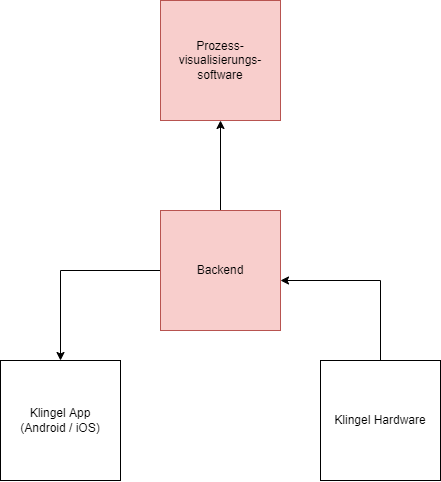
\includegraphics[width=\paperwidth/2]{../assets/img/kontextmodell}

    \caption{Kontextmodell der neu zu entwickelnden (Weiß) Komponenten in Verbindung zu bestehenden (Rot) Komponenten}
    \label{fig:kontextmodell}
\end{figure}
In Abbildung~\ref{fig:kontextmodell} ist das Kontextmodell dargestellt.
Bestandssysteme sind dabei in Rot dargestellt.
Hinzugefügt werden Apps für Android sowie iOS Apps und die Hardware für die Klingel.
Diese werden an das vorhandene Backend angebunden, welches entsprechend erweitert wird.